% =========================================================================
% BÀI 32: PHÉP TRỪ SỐ CÓ HAI CHỮ SỐ CHO SỐ CÓ HAI CHỮ SỐ (KHÔNG NHỚ)
% TOÀN BỘ CÂU HỎI ĐƯỢC VẼ HÌNH MINH HỌA TRỰC QUAN 100% BẰNG TIKZ 2D & 3D
% =========================================================================

% --- CÁC HÀM VẼ HÌNH TRỰC QUAN ĐẶC TRƯNG CHO BÀI 32 ---

% 1. Mô hình đặt tính trừ 2 số có 2 chữ số theo cột dọc
\providecommand{\VeDatTinhTruHaiSo}[4]{% #1=(x,y), #2=số bị trừ, #3=số trừ, #4=hiệu
  \begin{scope}[shift={(#1)}, scale=0.7]
    \draw[fill=blue!5, draw=blue!70, line width=0.8pt, rounded corners=3pt] (-1.1,-1.2) rectangle (1.1,1.2);
    \node[font=\bfseries\Large, color=black] at (0.3,0.6) {#2};
    \node[font=\bfseries\Large, color=red!85] at (-0.6,0.0) {$-$};
    \node[font=\bfseries\Large, color=black] at (0.3,0.0) {#3};
    \draw[line width=1.2pt, black!80] (-0.8,-0.3) -- (0.8,-0.3);
    \node[font=\bfseries\Large, color=blue!90!black] at (0.3,-0.75) {#4};
  \end{scope}
}

% 2. Thanh chục và khối đơn vị bị gạch chéo cả chục lẫn đơn vị
\providecommand{\VeKhoiTruHaiSo}[5]{% #1=(x,y), #2=tổng chục, #3=chục gạch bớt, #4=tổng đv, #5=đv gạch bớt
  \begin{scope}[shift={(#1)}, scale=0.42]
    % Vẽ các thanh chục
    \foreach \c in {1,...,#2} {
      \draw[fill=orange!50, draw=black!80, line width=0.4pt] (\c*0.7-0.7,0) rectangle (\c*0.7-0.2,2.8);
      \foreach \y in {0.28,0.56,...,2.6} {
        \draw[black!50, line width=0.2pt] (\c*0.7-0.7,\y) -- (\c*0.7-0.2,\y);
      }
      % Gạch chéo nếu nằm trong số chục bớt
      \ifnum\c>#2-#3
        \draw[line width=1.1pt, red!85] (\c*0.7-0.7,0) -- (\c*0.7-0.2,2.8);
        \draw[line width=1.1pt, red!85] (\c*0.7-0.7,2.8) -- (\c*0.7-0.2,0);
      \fi
    }
    % Vẽ các khối đơn vị
    \pgfmathsetmacro{\xstart}{#2*0.7 + 0.3}
    \foreach \u in {1,...,#4} {
      \draw[fill=cyan!50, draw=black!80, line width=0.4pt] (\xstart,\u*0.46-0.46) rectangle (\xstart+0.42,\u*0.46-0.05);
      \ifnum\u>#4-#5
        \draw[line width=1.0pt, red!85] (\xstart,\u*0.46-0.46) -- (\xstart+0.42,\u*0.46-0.05);
        \draw[line width=1.0pt, red!85] (\xstart,\u*0.46-0.05) -- (\xstart+0.42,\u*0.46-0.46);
      \fi
    }
  \end{scope}
}

% 3. Xe tải chở phép tính trừ hai số
\providecommand{\VeXePhepTruHaiSo}[4]{% #1=(x,y), #2=màu xe, #3=phép tính, #4=kết quả
  \begin{scope}[shift={(#1)}, scale=0.6]
    \draw[fill=#2!35, draw=black!80, line width=0.7pt, rounded corners=3pt] (-1.6,0) rectangle (1.6,0.9);
    \draw[fill=white, draw=black!70, line width=0.5pt, rounded corners=2pt] (-1.4,0.15) rectangle (1.4,0.75);
    \node[font=\bfseries\small, color=blue!90!black] at (0,0.45) {#3 = #4};
    \fill[black!85] (-1.0,-0.12) circle (0.2cm);
    \fill[gray!40] (-1.0,-0.12) circle (0.09cm);
    \fill[black!85] (1.0,-0.12) circle (0.2cm);
    \fill[gray!40] (1.0,-0.12) circle (0.09cm);
  \end{scope}
}

% =========================================================================
% BẮT ĐẦU NỘI DUNG 20 CÂU HỎI
% =========================================================================

\textbf{Phần 1. Trắc nghiệm lựa chọn}
\setcounterpageref{ex}{0}

% --- TRANG 1: CÂU 1 ĐẾN CÂU 4 ---

% CÂU 1: 56 - 23 bằng mô hình khối
\begin{ex} %[1D8N32]
Mô hình gồm $5$ thanh chục và $6$ khối đơn vị, bị bớt đi $2$ thanh chục và $3$ khối đơn vị:
\begin{center}\vspace{-2.5mm}
\begin{tikzpicture}
  \VeKhoiTruHaiSo{0,0}{5}{2}{6}{3}
  \node[below, font=\bfseries\tiny, color=blue!90!black] at (1.8,-0.2) {Ban đầu: $56$};
  \node[below, font=\bfseries\tiny, color=red!85] at (4.5,-0.2) {Bớt: $23$};
\end{tikzpicture}
\vspace{-2.5mm}\end{center}
Kết quả của phép tính $56 - 23$ là:
\begin{multicols}{4}
\choice
{$32$}
{\True $33$}
{$34$}
{$35$}
\end{multicols}
\loigiai{
Hàng đơn vị: $6 - 3 = 3$. Hàng chục: $5 - 2 = 3$. Vậy $56 - 23 = 33$.\\
\textbf{Đáp án: B.}
}
\end{ex}

% CÂU 2: Trừ tròn chục 70 - 30
\begin{ex} %[1D8N32]
Bác nông dân có $7$ bó que tính (mỗi bó $1$ chục), bác bán đi $3$ bó que tính:
\begin{center}\vspace{-2.5mm}
\begin{tikzpicture}[scale=0.5]
  \foreach \i in {1,...,7} {
    \draw[fill=teal!40, draw=teal!80, line width=0.6pt, rounded corners=2pt] (\i*1.1-1.1, 0) rectangle (\i*1.1-0.3, 1.3);
    \node[font=\bfseries\tiny, color=black] at (\i*1.1-0.7, 0.65) {$10$};
    \ifnum\i>4
      \draw[line width=1.2pt, red!85] (\i*1.1-1.1, 0) -- (\i*1.1-0.3, 1.3);
      \draw[line width=1.2pt, red!85] (\i*1.1-1.1, 1.3) -- (\i*1.1-0.3, 0);
    \fi
  }
  \node[above, font=\bfseries\scriptsize, color=red!85] at (5.9, 1.3) {Bán đi $30$};
  \node[above, font=\bfseries\scriptsize, color=teal!90!black] at (1.6, 1.3) {Còn lại $40$};
\end{tikzpicture}
\vspace{-2.5mm}\end{center}
Kết quả của phép tính $70 - 30$ là:
\begin{multicols}{4}
\choice
{$30$}
{$50$}
{$60$}
{\True $40$}
\end{multicols}
\loigiai{
$7$ chục trừ $3$ chục bằng $4$ chục. Vậy $70 - 30 = 40$.\\
\textbf{Đáp án: D.}
}
\end{ex}

% CÂU 3: Đặt tính 87 - 45
\begin{ex} %[1D8H32]
Quan sát phép tính đặt theo cột dọc:
\begin{center}\vspace{-2.5mm}
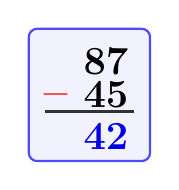
\begin{tikzpicture}
  \VeDatTinhTruHaiSo{0,0}{87}{45}{42}
\end{tikzpicture}
\vspace{-2.5mm}\end{center}
Kết quả của phép tính $87 - 45$ là:
\begin{multicols}{4}
\choice
{\True $42$}
{$41$}
{$43$}
{$44$}
\end{multicols}
\loigiai{
Hàng đơn vị: $7 - 5 = 2$. Hàng chục: $8 - 4 = 4$. Vậy kết quả là $42$.\\
\textbf{Đáp án: A.}
}
\end{ex}

% CÂU 4: Xe tải 98 - 64
\begin{ex} %[1D8H32]
Xe tải chở thùng hàng mang phép tính trừ:
\begin{center}\vspace{-2.5mm}
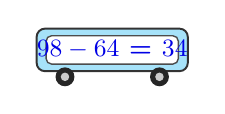
\begin{tikzpicture}
  \VeXePhepTruHaiSo{0,0}{cyan}{$98 - 64$}{$34$}
\end{tikzpicture}
\vspace{-2.5mm}\end{center}
Hiệu của hai số trên thùng xe tải là:
\begin{multicols}{4}
\choice
{$33$}
{$35$}
{\True $34$}
{$36$}
\end{multicols}
\loigiai{
Ta tính: $8 - 4 = 4$, $9 - 6 = 3$. Do đó $98 - 64 = 34$.\\
\textbf{Đáp án: C.}
}
\end{ex}

\newpage
% --- TRANG 2: CÂU 5 ĐẾN CÂU 8 ---

% CÂU 5: Cân đĩa tìm x + 23 = 68
\begin{ex} %[1D8H32]
Hai đĩa cân thăng bằng, đĩa trái có quả cân $68$, đĩa phải có quả cân $23$ và hộp quà $x$:
\begin{center}\vspace{-1mm}
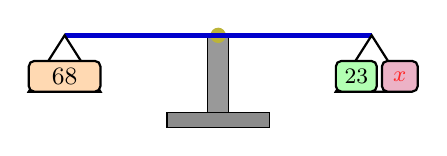
\begin{tikzpicture}[scale=0.65]
  % Trục cân
  \draw[fill=gray!80, draw=black] (-0.2,0) rectangle (0.2,1.8);
  \draw[fill=gray!90, draw=black] (-1.0,0) rectangle (1.0,0.3);
  \fill[yellow!70!black] (0,1.8) circle (0.15cm);
  \draw[line width=2pt, blue!80!black] (-3.0,1.8) -- (3.0,1.8);
  % Đĩa trái
  \draw[line width=0.8pt] (-3.0,1.8) -- (-3.7,0.7) -- (-2.3,0.7) -- cycle;
  \draw[fill=orange!30, line width=0.8pt, rounded corners=2pt] (-3.7,0.7) rectangle (-2.3,1.3);
  \node[font=\bfseries\small, color=black] at (-3.0,1.0) {$68$};
  % Đĩa phải
  \draw[line width=0.8pt] (3.0,1.8) -- (2.3,0.7) -- (3.7,0.7) -- cycle;
  \draw[fill=green!30, line width=0.8pt, rounded corners=2pt] (2.3,0.7) rectangle (3.1,1.3);
  \node[font=\bfseries\footnotesize, color=black] at (2.7,1.0) {$23$};
  \draw[fill=purple!30, line width=0.8pt, rounded corners=2pt] (3.2,0.7) rectangle (3.9,1.3);
  \node[font=\bfseries\footnotesize, color=red!85] at (3.55,1.0) {$x$};
\end{tikzpicture}
\vspace{-2mm}\end{center}
Giá trị của $x$ để hai đĩa cân bằng nhau là:
\begin{multicols}{4}
\choice
{$44$}
{\True $45$}
{$46$}
{$47$}
\end{multicols}
\loigiai{
Vì hai đĩa cân thăng bằng nên $x + 23 = 68$. Suy ra $x = 68 - 23 = 45$.\\
\textbf{Đáp án: B.}
}
\end{ex}

% CÂU 6: So sánh hai phép tính trừ
\begin{ex} %[1D8H32]
Hai chú sóc mang hai bảng phép tính:
\begin{center}\vspace{-1mm}
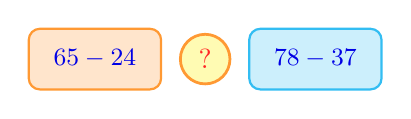
\begin{tikzpicture}[scale=0.7]
  % Bảng trái
  \draw[fill=orange!20, draw=orange!80, line width=0.8pt, rounded corners=4pt] (-3.2,-0.4) rectangle (-0.8,0.7);
  \node[font=\bfseries\small, color=blue!90!black] at (-2.0,0.15) {$65 - 24$};
  % Ô tròn so sánh
  \draw[fill=yellow!30, draw=orange!80, line width=1pt] (0,0.15) circle (0.45cm);
  \node[font=\bfseries\normalsize, color=red!85] at (0,0.15) {$?$};
  % Bảng phải
  \draw[fill=cyan!20, draw=cyan!80, line width=0.8pt, rounded corners=4pt] (0.8,-0.4) rectangle (3.2,0.7);
  \node[font=\bfseries\small, color=blue!90!black] at (2.0,0.15) {$78 - 37$};
\end{tikzpicture}
\vspace{-2mm}\end{center}
Dấu thích hợp điền vào dấu hỏi chấm ($?$) là:
\begin{multicols}{4}
\choice
{\True $=$}
{$>$}
{$<$}
{$+$}
\end{multicols}
\loigiai{
Ta có: $65 - 24 = 41$ và $78 - 37 = 41$. Vì $41 = 41$ nên dấu cần điền là dấu $=$.\\
\textbf{Đáp án: A.}
}
\end{ex}

% CÂU 7: Cuộn vải dài 85m cắt đi 32m
\begin{ex} %[1D8V32]
Một cuộn ruy băng dài $85\text{ cm}$, bạn Mai cắt đi một đoạn dài $32\text{ cm}$:
\begin{center}\vspace{-1mm}
\begin{tikzpicture}[scale=0.75]
  % Băng ruy băng
  \draw[fill=pink!40, draw=purple!80, line width=0.8pt] (0,0) rectangle (8.5,0.6);
  % Đoạn đã cắt
  \draw[fill=red!20, draw=red!80, line width=0.8pt] (0,0) rectangle (3.2,0.6);
  \node[font=\bfseries\footnotesize, color=red!85] at (1.6,0.3) {Đã cắt $32\text{ cm}$};
  \node[font=\bfseries\footnotesize, color=purple!90!black] at (5.85,0.3) {Còn lại $?\text{ cm}$};
  % Mũi tên cả đoạn
  \draw[<->, line width=0.7pt, black] (0,-0.3) -- (8.5,-0.3) node[midway, below, font=\bfseries\footnotesize] {Cả cuộn: $85\text{ cm}$};
\end{tikzpicture}
\vspace{-2mm}\end{center}
Đoạn ruy băng còn lại dài là:
\begin{multicols}{4}
\choice
{$52\text{ cm}$}
{\True $53\text{ cm}$}
{$54\text{ cm}$}
{$55\text{ cm}$}
\end{multicols}
\loigiai{
Đoạn ruy băng còn lại là: $85 - 32 = 53\text{ cm}$.\\
\textbf{Đáp án: B.}
}
\end{ex}

% CÂU 8: Đàn gà 68 con, bán 25 con
\begin{ex} %[1D8V32]
Trang trại nuôi $68$ con gà, người ta đã xuất chuồng bán đi $25$ con gà:
\begin{center}\vspace{-1mm}
\begin{tikzpicture}[scale=0.7]
  \draw[fill=yellow!15, draw=orange!80, line width=0.8pt, rounded corners=6pt] (-3.8,-0.5) rectangle (3.8,0.7);
  \node[font=\bfseries\footnotesize, color=blue!90!black] at (-2.0, 0.1) {Có tất cả: $68$ con gà};
  \node[font=\bfseries\footnotesize, color=red!85] at (2.0, 0.1) {Đã bán: $25$ con gà};
\end{tikzpicture}
\vspace{-2mm}\end{center}
Trang trại còn lại số con gà là:
\begin{multicols}{4}
\choice
{$42$ con}
{$44$ con}
{\True $43$ con}
{$45$ con}
\end{multicols}
\loigiai{
Số con gà còn lại là: $68 - 25 = 43$ (con gà).\\
\textbf{Đáp án: C.}
}
\end{ex}

\newpage
% --- TRANG 3: CÂU 9 ĐẾN CÂU 12 ---

% CÂU 9: Trừ liên tiếp 96 - 42 - 21
\begin{ex} %[1D8V32]
Đường đi của chú ong mật qua các bông hoa phép tính:
\begin{center}\vspace{-1mm}
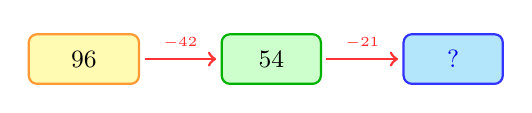
\begin{tikzpicture}[scale=0.7]
  % Bông hoa 1
  \draw[fill=yellow!30, draw=orange!80, line width=0.8pt, rounded corners=3pt] (-3.5,-0.4) rectangle (-1.5,0.5);
  \node[font=\bfseries\small, color=black] at (-2.5,0.05) {$96$};
  % Mũi tên 1
  \draw[->, line width=1pt, red!80] (-1.4,0.05) -- (-0.1,0.05) node[midway, above, font=\bfseries\tiny, color=red!85] {$-42$};
  % Bông hoa 2
  \draw[fill=green!20, draw=green!70!black, line width=0.8pt, rounded corners=3pt] (0.0,-0.4) rectangle (1.8,0.5);
  \node[font=\bfseries\small, color=black] at (0.9,0.05) {$54$};
  % Mũi tên 2
  \draw[->, line width=1pt, red!80] (1.9,0.05) -- (3.2,0.05) node[midway, above, font=\bfseries\tiny, color=red!85] {$-21$};
  % Đích đến
  \draw[fill=cyan!30, draw=blue!80, line width=0.8pt, rounded corners=3pt] (3.3,-0.4) rectangle (5.1,0.5);
  \node[font=\bfseries\small, color=blue!90!black] at (4.2,0.05) {$?$};
\end{tikzpicture}
\vspace{-2mm}\end{center}
Giá trị thích hợp điền vào ô hỏi chấm ($?$) là:
\begin{multicols}{4}
\choice
{$32$}
{$34$}
{\True $33$}
{$35$}
\end{multicols}
\loigiai{
Thực hiện từ trái sang phải: $96 - 42 = 54$, sau đó $54 - 21 = 33$.\\
\textbf{Đáp án: C.}
}
\end{ex}

% CÂU 10: Máy trừ 75 - y = 31
\begin{ex} %[1D8V32]
Một máy trừ nhận số đầu vào $75$, trừ đi số bí mật $y$ và cho kết quả $31$:
\begin{center}\vspace{-1mm}
\begin{tikzpicture}[scale=0.7]
  \node[font=\bfseries\small, color=blue!90!black] at (-3.0,0.4) {Đầu vào: $75$};
  \draw[->, line width=1.2pt, blue!80] (-1.7,0.4) -- (-0.8,0.4);
  \draw[fill=purple!20, draw=purple!80, line width=1pt, rounded corners=5pt] (-0.8,-0.2) rectangle (1.2,1.0);
  \node[font=\bfseries\small, color=red!85] at (0.2,0.4) {$- y$};
  \draw[->, line width=1.2pt, green!70!black] (1.2,0.4) -- (2.1,0.4);
  \node[font=\bfseries\small, color=green!60!black] at (3.3,0.4) {Kết quả: $31$};
\end{tikzpicture}
\vspace{-2mm}\end{center}
Số bí mật $y$ trong chiếc máy là:
\begin{multicols}{4}
\choice
{$43$}
{$45$}
{$46$}
{\True $44$}
\end{multicols}
\loigiai{
Số trừ $y = 75 - 31 = 44$.\\
\textbf{Đáp án: D.}
}
\end{ex}

% CÂU 11: So sánh nhãn vở của Mai và Lan
\begin{ex} %[1D8V32]
Biểu đồ số nhãn vở của hai bạn Mai và Lan:
\begin{center}\vspace{-1mm}
\begin{tikzpicture}[scale=0.75]
  \draw[fill=blue!30, draw=blue!80, line width=0.7pt] (0,0.8) rectangle (4.8,1.3);
  \node[left, font=\bfseries\footnotesize] at (0,1.05) {Mai:};
  \node[right, font=\bfseries\footnotesize, color=blue!90!black] at (4.8,1.05) {$48$ cái};
  \draw[fill=orange!30, draw=orange!80, line width=0.7pt] (0,0.1) rectangle (2.6,0.6);
  \node[left, font=\bfseries\footnotesize] at (0,0.35) {Lan:};
  \node[right, font=\bfseries\footnotesize, color=orange!90!black] at (2.6,0.35) {$26$ cái};
  % Phần chênh lệch
  \draw[dashed, line width=0.8pt, red!85] (2.6,0.1) -- (2.6,1.4);
  \draw[<->, line width=0.8pt, red!85] (2.6,0.7) -- (4.8,0.7) node[midway, above, font=\bfseries\tiny, color=red!85] {Nhiều hơn: $?$};
\end{tikzpicture}
\vspace{-2mm}\end{center}
Mai có nhiều hơn Lan số cái nhãn vở là:
\begin{multicols}{4}
\choice
{\True $22$ cái}
{$21$ cái}
{$23$ cái}
{$24$ cái}
\end{multicols}
\loigiai{
Mai nhiều hơn Lan số nhãn vở là: $48 - 26 = 22$ (cái).\\
\textbf{Đáp án: A.}
}
\end{ex}

% CÂU 12: Hiệu của 99 và 45
\begin{ex} %[1D8C32]
Đóa hoa mang phép tính hiệu giữa số lớn nhất có $2$ chữ số và số $45$:
\begin{center}\vspace{-1mm}
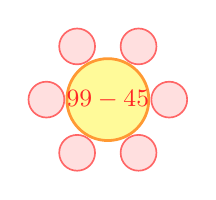
\begin{tikzpicture}[scale=0.65]
  \draw[fill=yellow!40, draw=orange!80, line width=1pt] (0,0) circle (0.8cm);
  \node[font=\bfseries\small, color=red!85] at (0,0) {$99 - 45$};
  \foreach \angle in {0,60,120,180,240,300} {
    \draw[fill=pink!50, draw=red!60, line width=0.6pt] (\angle:1.2) circle (0.35cm);
  }
\end{tikzpicture}
\vspace{-2mm}\end{center}
Hiệu của số lớn nhất có hai chữ số ($99$) và số $45$ là:
\begin{multicols}{4}
\choice
{$53$}
{$55$}
{$56$}
{\True $54$}
\end{multicols}
\loigiai{
Số lớn nhất có hai chữ số là $99$. Hiệu là: $99 - 45 = 54$.\\
\textbf{Đáp án: D.}
}
\end{ex}

\newpage
% --- TRANG 4: PHẦN 2 - TRẮC NGHIỆM ĐÚNG SAI (4 CÂU) ---

\textbf{Phần 2. Trắc nghiệm đúng sai}
\setcounterpageref{ex}{0}

% CÂU 13: Đặt tính trừ đúng hay sai
\begin{ex} %[1D8H32]
Xét tính đúng, sai của các kết quả phép trừ sau:
\begin{center}\vspace{-2mm}
\begin{tikzpicture}[scale=0.7]
  \node at (-4.5,0) {\VeDatTinhTruHaiSo{0,0}{67}{25}{42}};
  \node at (-1.5,0) {\VeDatTinhTruHaiSo{0,0}{89}{53}{36}};
  \node at (1.5,0) {\VeDatTinhTruHaiSo{0,0}{74}{31}{45}};
  \node at (4.5,0) {\VeDatTinhTruHaiSo{0,0}{98}{64}{34}};
\end{tikzpicture}
\vspace{-2mm}\end{center}
\choiceTF
{\True $67 - 25 = 42$}
{\True $89 - 53 = 36$}
{$74 - 31 = 45$}
{\True $98 - 64 = 34$}
\loigiai{
\begin{itemize}
    \item a) Đúng vì $7 - 5 = 2$, $6 - 2 = 4$.
    \item b) Đúng vì $9 - 3 = 6$, $8 - 5 = 3$.
    \item c) Sai vì $74 - 31 = 43 \neq 45$.
    \item d) Đúng vì $8 - 4 = 4$, $9 - 6 = 3$.
\end{itemize}
}
\end{ex}

% CÂU 14: Bao gạo cửa hàng
\begin{ex} %[1D8V32]
Một cửa hàng lương thực có $95\text{ kg}$ gạo. Trong buổi sáng, cửa hàng đã bán được $42\text{ kg}$ gạo:
\begin{center}\vspace{-2mm}
\begin{tikzpicture}[scale=0.7]
  \draw[fill=amber!25, draw=brown!80, line width=0.8pt, rounded corners=5pt] (-3.8,-0.5) rectangle (3.8,0.7);
  \node[font=\bfseries\footnotesize, color=blue!90!black] at (-2.0, 0.1) {Có tất cả: $95\text{ kg}$ gạo};
  \node[font=\bfseries\footnotesize, color=red!85] at (2.0, 0.1) {Đã bán: $42\text{ kg}$ gạo};
\end{tikzpicture}
\vspace{-2mm}\end{center}
Xét tính đúng, sai của các nhận xét sau:
\choiceTF
{\True Sau buổi sáng, cửa hàng còn lại $53\text{ kg}$ gạo.}
{Cửa hàng còn lại $50\text{ kg}$ gạo.}
{\True Số gạo còn lại nhiều hơn số gạo đã bán là $11\text{ kg}$.}
{Số gạo đã bán nhiều hơn số gạo còn lại.}
\loigiai{
\begin{itemize}
    \item a) Đúng: Số gạo còn lại là $95 - 42 = 53\text{ kg}$.
    \item b) Sai: Còn lại $53\text{ kg}$, không phải $50\text{ kg}$.
    \item c) Đúng: $53 - 42 = 11\text{ kg}$.
    \item d) Sai: $53 > 42$ nên số gạo còn lại nhiều hơn số gạo đã bán.
\end{itemize}
}
\end{ex}

% CÂU 15: So sánh các phép trừ
\begin{ex} %[1D8H32]
Cho các phép tính trừ được viết trên các tấm thẻ số:
\begin{center}\vspace{-2mm}
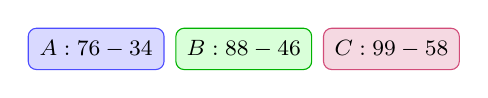
\begin{tikzpicture}[scale=0.75]
  \draw[fill=blue!15, draw=blue!70, rounded corners=3pt] (-3.5,0) rectangle (-1.2,0.7) node[midway, font=\bfseries\footnotesize] {$A: 76 - 34$};
  \draw[fill=green!15, draw=green!70!black, rounded corners=3pt] (-1.0,0) rectangle (1.3,0.7) node[midway, font=\bfseries\footnotesize] {$B: 88 - 46$};
  \draw[fill=purple!15, draw=purple!70, rounded corners=3pt] (1.5,0) rectangle (3.8,0.7) node[midway, font=\bfseries\footnotesize] {$C: 99 - 58$};
\end{tikzpicture}
\vspace{-2mm}\end{center}
Xét tính đúng, sai của các khẳng định sau:
\choiceTF
{\True Phép tính $A$ có kết quả là $42$.}
{\True Phép tính $B$ có kết quả là $42$.}
{\True Phép tính $A$ và phép tính $B$ có kết quả bằng nhau.}
{Phép tính $C$ có kết quả lớn hơn phép tính $B$.}
\loigiai{
\begin{itemize}
    \item a) Đúng vì $76 - 34 = 42$.
    \item b) Đúng vì $88 - 46 = 42$.
    \item c) Đúng vì cả hai phép tính đều có kết quả là $42$.
    \item d) Sai vì phép tính $C = 99 - 58 = 41 < 42$ (kết quả của $C$ bé hơn $B$).
\end{itemize}
}
\end{ex}

% CÂU 16: Bảng hoa điểm tốt của hai tổ
\begin{ex} %[1D8V32]
Bảng thống kê số bông hoa điểm tốt của hai tổ trong tháng:
\begin{center}\vspace{-2mm}
\begin{tikzpicture}[scale=0.75]
  \draw[fill=teal!15, draw=teal!80, line width=0.8pt] (0,0) rectangle (7.0,1.2);
  \draw[line width=0.6pt, teal!80] (0,0.6) -- (7.0,0.6);
  \draw[line width=0.6pt, teal!80] (3.5,0) -- (3.5,1.2);
  \node[font=\bfseries\footnotesize] at (1.75,0.9) {Tổ 1: $48$ bông hoa};
  \node[font=\bfseries\footnotesize] at (5.25,0.9) {Tổ 2: $36$ bông hoa};
  \node[font=\bfseries\footnotesize, color=teal!90!black] at (3.5,0.3) {Tổng số hoa cả hai tổ: $84$ bông};
\end{tikzpicture}
\vspace{-2mm}\end{center}
Xét tính đúng, sai của các nhận định:
\choiceTF
{\True Tổ 1 có nhiều hơn Tổ 2 là $12$ bông hoa điểm tốt.}
{Tổ 2 có nhiều hơn Tổ 1 bông hoa điểm tốt.}
{\True Nếu Tổ 2 có thêm $12$ bông hoa thì số hoa hai tổ sẽ bằng nhau.}
{Hiệu số bông hoa giữa Tổ 1 và Tổ 2 là $14$ bông hoa.}
\loigiai{
\begin{itemize}
    \item a) Đúng: $48 - 36 = 12$ bông hoa.
    \item b) Sai: Vì $48 > 36$ nên Tổ 1 nhiều hơn Tổ 2.
    \item c) Đúng: $36 + 12 = 48$ bằng số hoa của Tổ 1.
    \item d) Sai: Hiệu số hoa là $12$, không phải $14$.
\end{itemize}
}
\end{ex}

\newpage
% --- TRANG 5: PHẦN 3 - CÂU HỎI TRẢ LỜI NGẮN (4 CÂU) ---

\textbf{Phần 3. Câu hỏi trả lời ngắn}
\setcounterpageref{ex}{0}

% CÂU 17: Tính 68 - 35
\begin{ex} %[1D8H32]
Tính giá trị của phép tính trừ: $68 - 35$.
\begin{center}\vspace{-2mm}
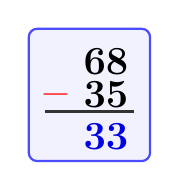
\begin{tikzpicture}
  \VeDatTinhTruHaiSo{0,0}{68}{35}{33}
\end{tikzpicture}
\vspace{-2mm}\end{center}
Kết quả của phép tính là bao nhiêu?
\textit{Trả lời:} \raisebox{-2pt}{\tcbox[colframe=blue!80!black,colback=white,size=small,arc=3pt]{$33$}}
\loigiai{
Đơn vị: $8 - 5 = 3$; Hàng chục: $6 - 3 = 3$. Vậy $68 - 35 = 33$.\\
\textbf{Đáp số: $33$.}
}
\end{ex}

% CÂU 18: Tìm x trong phép cộng x + 34 = 78
\begin{ex} %[1D8V32]
Ngôi nhà toán học có tổng hai số ở tầng dưới bằng số ở mái nhà:
\begin{center}\vspace{-2mm}
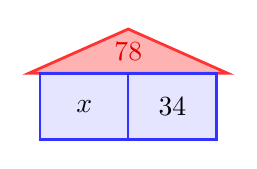
\begin{tikzpicture}[scale=0.7]
  % Mái nhà
  \draw[fill=red!30, draw=red!80, line width=1pt] (0,1.2) -- (-1.8,0.4) -- (1.8,0.4) -- cycle;
  \node[font=\bfseries\normalsize, color=red!90!black] at (0,0.8) {$78$};
  % Thân nhà
  \draw[fill=blue!10, draw=blue!80, line width=1pt] (-1.6,0.4) rectangle (1.6,-0.8);
  \draw[line width=0.8pt, blue!80] (0,0.4) -- (0,-0.8);
  \node[font=\bfseries\normalsize, color=black] at (-0.8,-0.2) {$x$};
  \node[font=\bfseries\normalsize, color=black] at (0.8,-0.2) {$34$};
\end{tikzpicture}
\vspace{-2mm}\end{center}
Tìm số $x$ biết $x + 34 = 78$.
\textit{Trả lời:} \raisebox{-2pt}{\tcbox[colframe=blue!80!black,colback=white,size=small,arc=3pt]{$44$}}
\loigiai{
Ta có $x = 78 - 34 = 44$.\\
\textbf{Đáp số: $44$.}
}
\end{ex}

% CÂU 19: Bài toán số bạn nữ trong lớp
\begin{ex} %[1D8V32]
Lớp 1A có tất cả $38$ học sinh, trong đó có $15$ bạn nam:
\begin{center}\vspace{-2mm}
\begin{tikzpicture}[scale=0.7]
  \draw[fill=green!20, draw=green!70!black, line width=0.8pt, rounded corners=4pt] (-3.5,-0.4) rectangle (3.5,0.6);
  \node[font=\bfseries\footnotesize, color=blue!90!black] at (-1.8,0.1) {Cả lớp: $38$ bạn};
  \node[font=\bfseries\footnotesize, color=teal!90!black] at (1.8,0.1) {Nam: $15$ bạn $\to$ Nữ: $?$};
\end{tikzpicture}
\vspace{-2mm}\end{center}
Hỏi lớp 1A có bao nhiêu bạn nữ?
\textit{Trả lời:} \raisebox{-2pt}{\tcbox[colframe=blue!80!black,colback=white,size=small,arc=3pt]{$23$}}
\loigiai{
Số bạn nữ của lớp 1A là: $38 - 15 = 23$ (bạn).\\
\textbf{Đáp số: $23$ bạn.}
}
\end{ex}

% CÂU 20: Tìm hiệu số lớn nhất hàng chục là 8 và 42
\begin{ex} %[1D8C32]
Chiếc rương kho báu mang câu đố:
\begin{center}\vspace{-2mm}
\begin{tikzpicture}[scale=0.75]
  \draw[fill=yellow!30, draw=orange!90, line width=1pt, rounded corners=4pt] (-3.0,-0.5) rectangle (3.0,0.7);
  \node[font=\bfseries\footnotesize, color=red!85] at (0,0.3) {Số lớn nhất hàng chục bằng $8$: $89$};
  \node[font=\bfseries\footnotesize, color=blue!90!black] at (0,-0.15) {Trừ đi $42 \implies 89 - 42 = ?$};
\end{tikzpicture}
\vspace{-2mm}\end{center}
Tìm hiệu của số lớn nhất có hai chữ số có hàng chục bằng $8$ với số $42$.
\textit{Trả lời:} \raisebox{-2pt}{\tcbox[colframe=blue!80!black,colback=white,size=small,arc=3pt]{$47$}}
\loigiai{
Số lớn nhất có hàng chục bằng $8$ là $89$. Hiệu cần tìm: $89 - 42 = 47$.\\
\textbf{Đáp số: $47$.}
}
\end{ex}
